\documentclass{MScthesisITEM}

% this package is just to generate text for demo-purposes
\usepackage{blindtext}
\usepackage{todonotes}


\title{ Visualization of large scale Netflow data} % The title of your assignement; NB use \newlinetitle to start a newline
\author{Nicolai Eeg-Larsen} % Your firstname and lastname
\professor{Firstname Lastname, Affiliation} % Affiliation = ITEM for instance
\supervisor{Firstname Lastname, Affiliation}

%% Uncomment the following in case you want subfigures; note that there will be a warning for the caption package
% \let\subcaption\undefined
% \let\subfloat\undefined
% \usepackage[bf]{caption}
% \usepackage{subcaption}

\DeclareGraphicsExtensions{.pdf,.jpg, .png}
\graphicspath{{./figs/}}

\loadglsentries{glossary}
\makeglossaries

\begin{document}
\selectlanguage{english}
\pagenumbering{roman}
\pagestyle{plain}

%% Only for the project; comment out the line below for the master's thesis; the front page will be generated automatically by DAIM
\titleITEM

%% Only for the master's thesis; for the project report the description is taken from It's Learning and added by the department
% \selectlanguage{english} % Change to 'norsk' if you are writing in Norwegian
% \begin{titlingpage}

\noindent
\begin{tabular}{@{}p{4cm}l}
\textbf{Title:} 	& \thetitle \\
\textbf{Student:}	& \theauthor \\
\end{tabular}

\vspace{4ex}
\noindent\textbf{Problem description:}
\vspace{2ex}

\noindent \Blindtext[2][1]
\vspace{6ex}

\noindent
\begin{tabular}{@{}p{4cm}l}
\textbf{Responsible professor:} 	& \theprofessor \\
\textbf{Supervisor:}			& \thesupervisor \\
\end{tabular}

\end{titlingpage}
% \cleardoublepage

%% There must be an abstract in English, even though the main text is in Norwegian
\selectlanguage{english}
\cleardoublepage

%% Only for the master's thesis; if the main text is in English and you can write Norwegian, there must be an abstract in Norwegian as well.
% \selectlanguage{norsk}
% \pagestyle{empty}
\renewcommand{\abstractname}{Sammendrag}
\begin{abstract}
\noindent Sikkerheten til nesten all offentlig nøkkel-kryptografi er basert på et vanskelig beregnbarhetsproblem. Mest velkjent er problemene med å faktorisere heltall i sine primtallsfaktorer, og å beregne diskrete logaritmer i endelige sykliske grupper. I de to siste tiårene, har det imidlertid dukket opp en rekke andre offentlig nøkkel-systemer, som baserer sin sikkerhet på helt andre type problemer. Et lovende forslag, er å basere sikkerheten på vanskeligheten av å løse store likningsett av flervariable polynomlikninger. En stor utfordring ved å designe slike offentlig nøkkel-systemer, er å integrere en effektiv ``falluke'' (trapdoor) inn i likningssettet. En ny tilnærming til dette problemet ble nylig foreslått av Gligoroski m.f., hvor de benytter konseptet om kvasigruppe-strengtransformasjoner (quasigroup string transformations). I denne masteroppgaven beskriver vi en metodikk for å identifisere sterke og svake nøkler i det nylig foreslåtte multivariable offentlig nøkkel-signatursystemet MQQ-SIG, som er basert på denne idéen.

Vi har gjennomført et stort antall eksperimenter, basert på Gröbner basis angrep, for å klassifisere de ulike parametrene som bestemmer nøklene i MQQ-SIG. Våre funn viser at det er store forskjeller i viktigheten av disse parametrene. Metodikken består i en klassifisering av de forskjellige parametrene i systemet, i tillegg til en innføring av konkrete kriterier for hvilke nøkler som bør velges. Videre, har vi identifisert et unødvendig krav i den originale spesifikasjonen, som krevde at kvasigruppene måtte oppfylle et bestemt kriterie. Ved å fjerne denne betingelsen, kan nøkkel-genererings-algoritmen potensielt øke ytelsen med en stor faktor. Basert på alt dette, foreslår vi en ny og forbedret nøkkel-genereringsalgoritme for MQQ-SIG, som vil generere sterkere nøkler og være mer effektiv enn den originale nøkkel-genereringsalgoritmen.  
\end{abstract}
% \cleardoublepage

\selectlanguage{english}% Change to 'norsk' if you are writing in Norwegian

\renewcommand{\abstractname}{Preface}
\begin{abstract}
\noindent \blindtext 
\end{abstract}
\cleardoublepage

% similarly you may add a separate acknowledgments page

\tableofcontents*
\cleardoublepage

%% include if relevant
\listoffigures
\cleardoublepage

%% include if relevant
\listoftables
\cleardoublepage

%% include if relevant
\listofalgorithms
\addcontentsline{toc}{chapter}{List of Algorithms}
\cleardoublepage

%% include if relevant
\printglossary[title=List of Symbols, style=long]
\cleardoublepage
\glsaddall[]

%% include if relevant
\printglossary[title=List of Acronyms,type=\acronymtype] % prints just the list of acronyms
\cleardoublepage

\pagenumbering{arabic}
\pagestyle{ruled}
\chapter{Background}
\label{chp:background} 

\section{NetFlow}
\label{netflow}
Cisco IOS NetFlow creates an enviroment that have the tools to understand who, what, when, where and how network traffic is flowing. This makes it easier for administrators to utilize the network as optimal as possible. One can determine the source and destination of traffic and use this information to reveal for example DDoS-attacks or spam mail.
\citep{flow_monitoring}
\todo{bruke den siste referansen}
\subsection{How does it work?}
Every packet that is forwarded within a router/switch is examined for a set of \gls{ip} packet attributes. With these attributes one can determine if the packet is unique or similar to other packets. 

The attributes used by NetFlow are:
\begin{itemize}
\item IP source address
\item IP destination address
\item Source port
\item Destination port
\item Layer 3 protocol type
\item Class of service
\item Router/Switch interface
\end{itemize}

To group packets into a flow, one compares source/destination IP address, source/destination ports, protocol interface and class of service. Then the packets and bytes are tallied. This method is scalable because a large amount of network information is condensed into a database of NetFlow information called the NetFlow cache. 

When the NetFlow cache is created one can use this to understand the network behaviour. The different attributes generate different knowledge about a certain network, and combined they can paint a detailed picture of how the network is working. For example the ports show what application is utilizing the traffic, while the tallied packets and bytes show the amount of traffic. 
\citep{cisco_netflow} \citep{netflow_evolve}

\begin{figure}[h!]
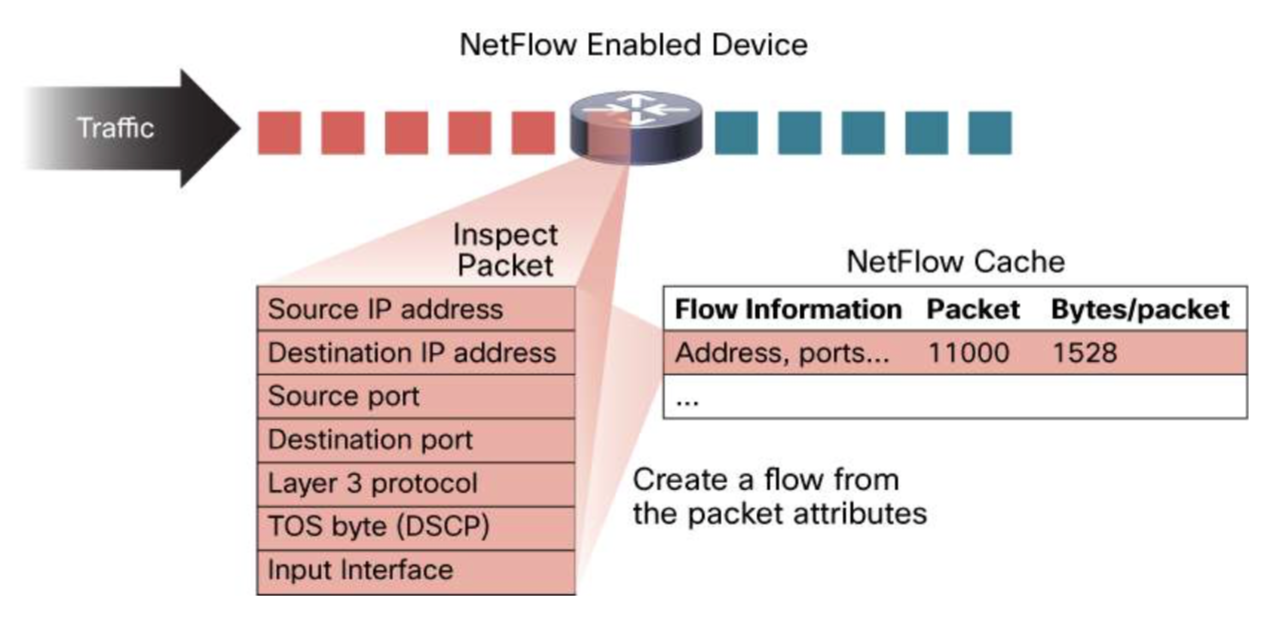
\includegraphics[scale=0.2]{netflow_cache}
\caption{Creating a flow in the NetFlow cache siter}
\end{figure}

\begin{itemize}
\item Source address allows the understanding of who is originating the traffic
\item Destination address tells who is receiving the traffic
\item Ports characterize the application utilizing the traffic
\item Class of service examines the priority of the traffic
\item The device interface tells how traffic is being utilized by the network device
\item Tallied packets and bytes show the amount of traffic
\end{itemize}

Additional information added to a flow includes:
\begin{itemize}


\item Flow timestamps to understand the life of a flow; timestamps are useful for calculating packets and bytes per second
\item Next hop IP addresses including \gls{bgp} routing \gls{as}
\item Subnet mask for the source and destination addresses to calculate prefixes
 \item  flags to examine \gls{tcp} handshakes

\end{itemize}
\todo{Lime inn hvordan det ser ut i kommandolinjen}

\todo{sitere listen}

\subsection{Main components}
A typical set-up using NetFlow consists of three main components:

\begin{itemize}
\item \textbf{Flow Exporter:} aggregates packets into flows and exports flow records towards one or more flow collectors. 

\item \textbf{Flow collector:} is responsible for reception, storage and pre-processing of flow data received from a flow exporter.

\item \textbf{Analysis application:} an application that analyse the received flow data in different contexts, such as intrusion or traffic profiling.
\end{itemize}

\begin{figure}[h!]
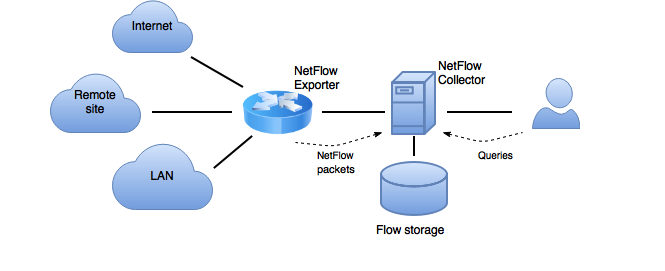
\includegraphics[scale=0.5]{netflow_arch}
\caption{Figure of a simple NetFlow architecture}
\end{figure}

\subsection{nfdump}
\todo(skrive om ipfix, v5 og v9, muligens i egen seksjon)
nfdump collect and process NetFlow data on the command line. It stores NetFlow data in time sliced files. The files are binary and this provides the possibility of either returning the output from nfdump in the same binary form, or as readable text. nfdump has four output formats, raw, line, long and extended. 
The challenge of representing \gls{ipv6} addresses is handled by shrinking them in the normal output. 
In figure \ref{nfdump_operation} the collection process is depicted, and in figure \ref{nfdump_processing} the processing of collected NetFlow data is shown.\citep{nfdump}

\begin{figure}[h!]
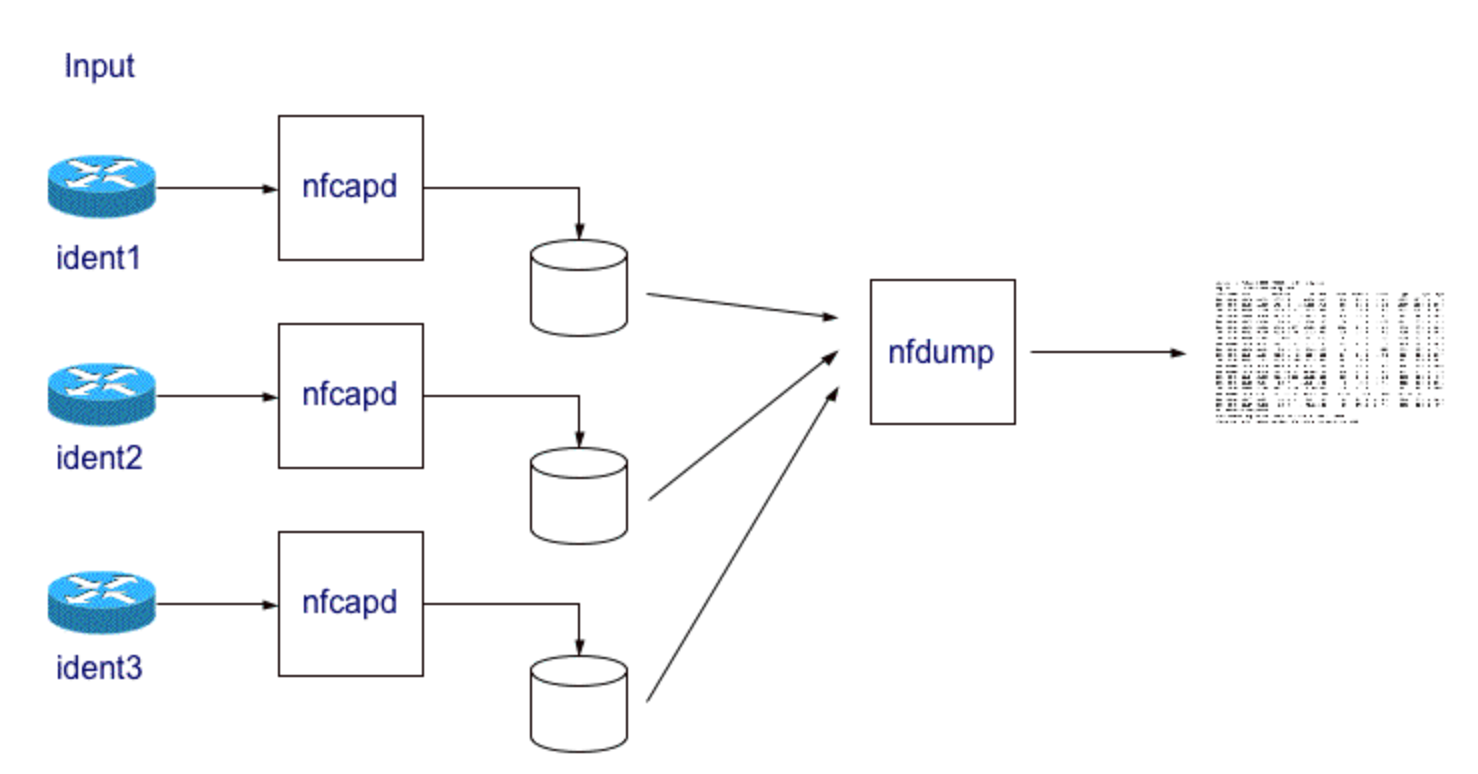
\includegraphics[scale=0.4]{nfdump_operation}
\caption{Example of dataset of random numbers where no pre-attentive processing is done}
\label{nfdump_operation}
\end{figure}

\begin{figure}[h!]
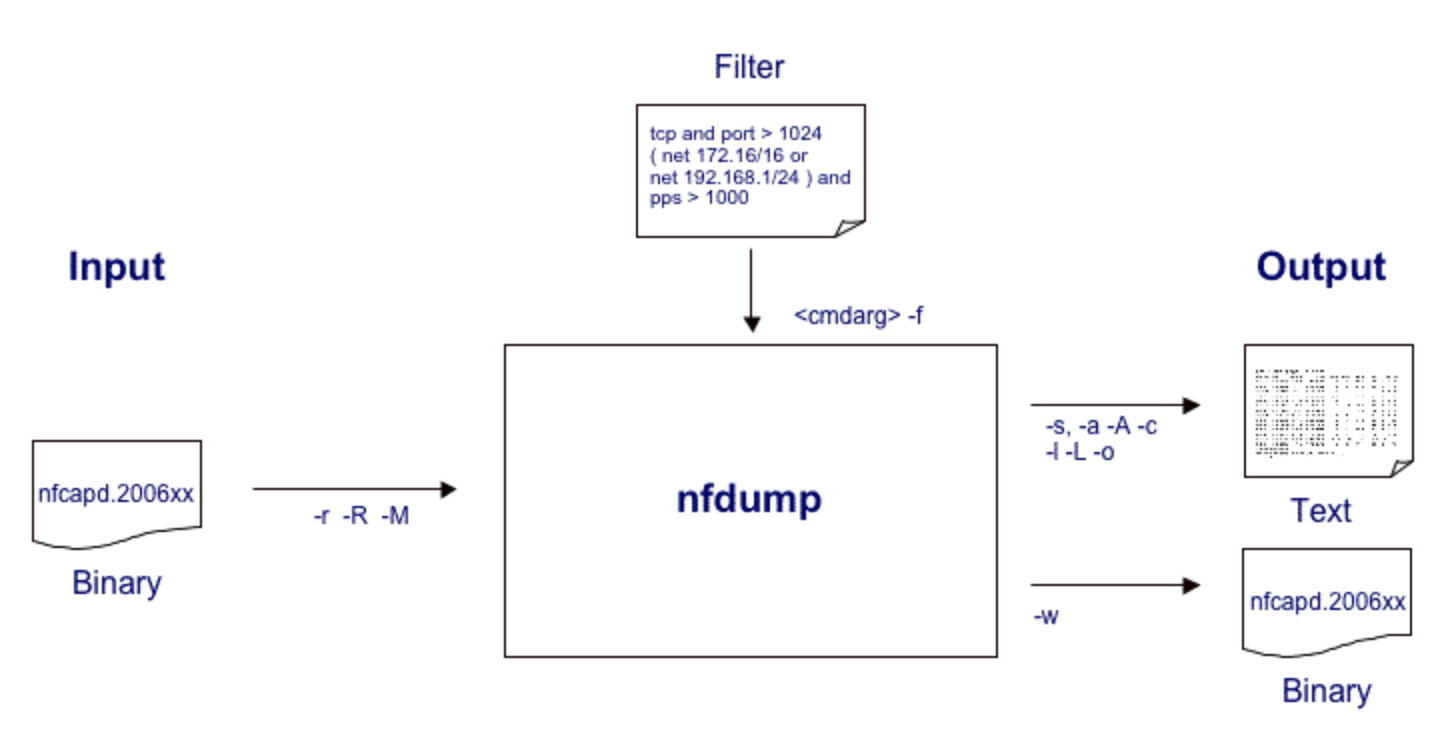
\includegraphics[scale=0.4]{nfdump2}
\caption{Example of dataset of random numbers where no pre-attentive processing is done}
\label{nfdump_processing}
\end{figure}

\subsubsection{v5,v9 and IPfix}
\begin{itemize}
\item \textbf{v5:} NetFlow v5 is definitely the most popular version of Cisco Netflow. It is fixed, meaning it always stays the same and makes for a simpler deciphering. 

\item \textbf{v9:} v9 is opposite of its predecessor dynamic. The collector will need to know the format of incoming NetFlow v9 flows, which means v9 templates periodically needs to be sent to the collector to inform of the format which the flows are being exported are. It was made to support technologies as Multi-cast, IPSec and Multi Protocol Label Switching (MPLS). This thanks to the templates. IPv6 support was added as well. \cite{v9}

\item \textbf{IPFIX:} Based on the design of NetFlow v9, \gls{ipfix} added support for variable length strings. Making it possible for Application Visibility and Control(AVC) exports in the future.\todo{forklare?} \cite{ipfix}
\end{itemize}

\subsubsection{Example of use}
An example of a nfdump command used in this project is for example how to extract the number of flows each day, and find the 10 most used destination IP-addresses:

\begin{lstlisting}[caption={nfdump example},label={lst:nfdumo}][language=bash]
nfdump -R /data/netflow/oslo_gw/2012/01/01/nfcapd.201201010000:nfcapd.201201012355 -n 10 -s dstip -o csv > example.csv
\end{lstlisting}

Such a request iterates over a number of files due to the -R command. In this case it is all captures between 00:00 until 23:55 on the first of January 2012. It is limited to the 10 most popular destination IP's with the -n and -s. All of this is stored in a .\gls{csv}file which is optimal for use with the D3.js framework. 

This results in the output shown in figure \ref{top10example}.

\begin{figure}[h!]
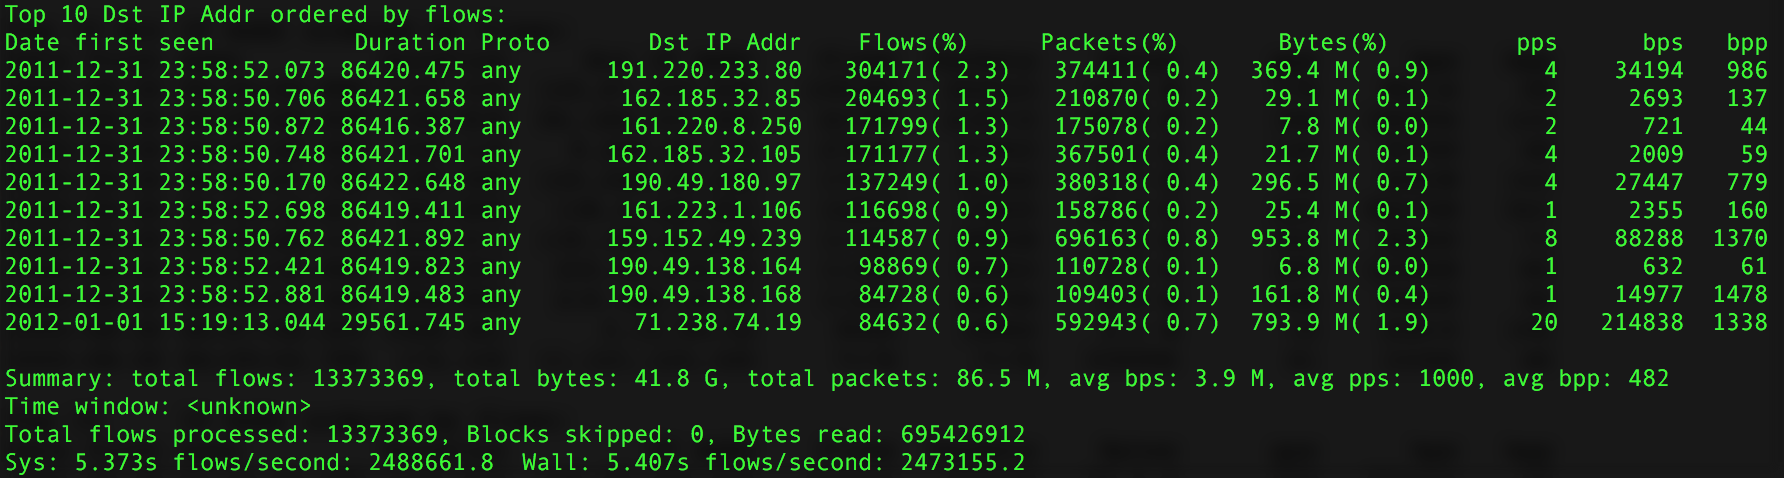
\includegraphics[scale=0.4]{top10example}
\caption{Example of dataset of random numbers where no pre-attentive processing is done}
\label{top10example}
\end{figure}



\section{Data visualization}
\label{sec:dataviz}
Data visualization refers to the techniques used to communicate data or information by encoding it as visual objects. Meaning that information is represented trough any visual element such as graphs and plots, but may also take any other visual form. Visualization helps users analyse and interact with data in a whole new way. It makes complex data more accessible, understandable and usable.\cite{friedman}

In recent years the rate of which data is generated has increased rapidly, and the need for information to be available and comprehensible is growing. All these new sources of data has created what we refer to as "Big Data" \cite{bigdata}. Without visual presentation such data is too big to understand. This is one of the major reasons visualization is emerging as a big market. 

Combining several parameters through visualization could reveal something automated systems might ignore or don't pick up on. \begin{quotation}
The greatest value of a picture is when it forces us to notice what we never expected to see.
\end{quotation} by John Tukey.

\subsection{Characteristics}
\label{characteristics}
In his book from 1983, The Visual Display of Quantitative Information\cite{tufte}, Edward Tufte defines characteristics any effective graphical representation should contain as:

\begin{itemize}
\item show the data
\item induce the viewer to think about the substance rather than about methodology, graphic design, the technology of graphic production or something else
\item avoid distorting what the data has to say
\item present many numbers in a small space
\item make large data sets coherent
\item encourage the eye to compare different pieces of data
\item reveal the data at several levels of detail, from a broad overview to the fine structure
\item serve a reasonably clear purpose: description, exploration, tabulation or decoration
\item be closely integrated with the statistical and verbal descriptions of a data set.
\end{itemize}

\subsection{Visual perception}
\label{sec:atentive}
In this paper the correlation between effective visual communication and how it is perceived upon human inspection is important. A humans ability to distinguish between differences in length, shape and color is referred to as "pre-attentive attributes".  

A good example of this is imagining finding the number of a certain character in a series of characters. This requires significant time and effort, but if the character were to stand out by being a different size, color or orientation this could be done quickly trough pre-attentive processing. Good data visualization takes all of this into consideration and uses pre-attentive processing. In this simple example it is easy to see how pre attentive processing is used to distinguish how many occurrences of the number 5 is in a larger set of random numbers. 
\newline

\begin{figure}[h!]
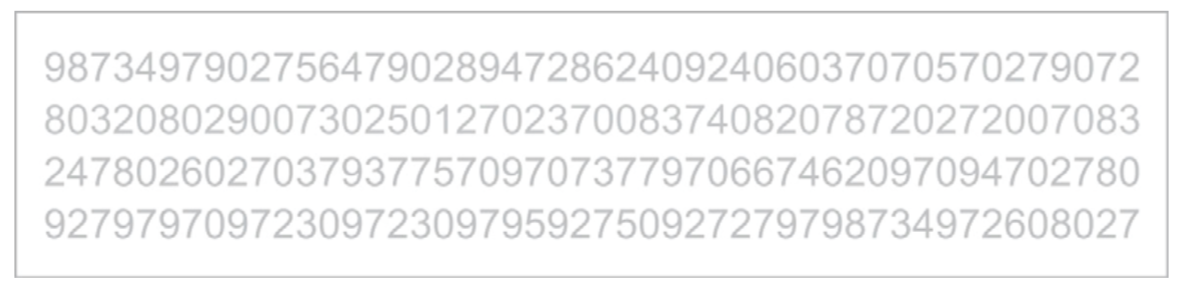
\includegraphics[scale=0.3]{attentive}
\caption{Example of dataset of random numbers where no pre-attentive processing is done}
\end{figure}

\begin{figure}[h!]
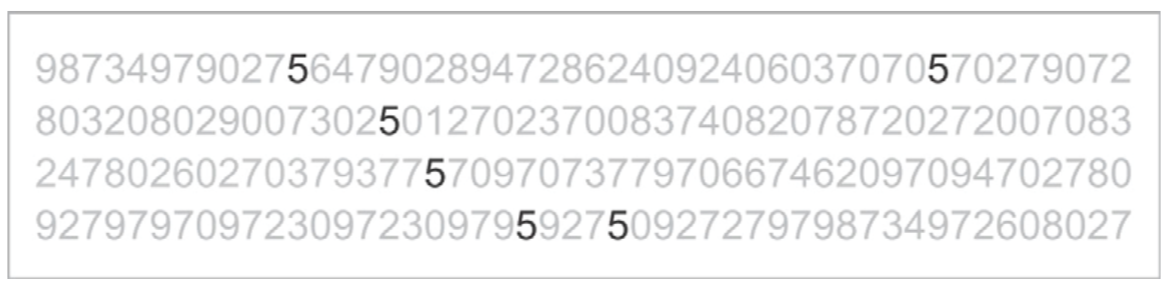
\includegraphics[scale=0.3]{pre_attentive}
\caption{Example of a dataset of random numbers where pre-attentive processing has been used to distinguish the occurrences of the number five}
\end{figure}
\subsection{Data presentation architecture}
\label{sec:dpa}
\gls{dpa} has its purpose to identify, locate, manipulate, format and present data in such a way as to optimally communicate meaning and proffer knowledge\cite{wiki_data_viz}. This has become an important tool in Business Intelligence, the art of transforming raw data into something useful. 

\subsubsection{Objectives}
DPA has two main objectives, which is the following:

\begin{itemize}
\item To use data to provide knowledge in the most efficient manner possible (minimize noise, complexity, and unnecessary data or detail given each audience's needs and roles)
\item To use data to provide knowledge in the most effective manner possible (provide relevant, timely and complete data to each audience member in a clear and understandable manner that conveys important meaning, is actionable and can affect understanding, behaviour and decisions)
\end{itemize}

\subsubsection{Scope}
The actual work of DPA consist of:
\begin{itemize}
\item Creating effective delivery mechanisms
\item Define relevant knowledge needed by each viewer
\item Determine how often the data should be updated
\item Determine how often and when the user needs to see the data
\item Finding the right data
\item Utilizing the best visualizations and presentation formats
\end{itemize}


\section{D3.js}
In this paper D3.js \citep{D3} is chosen as the framework to create examples of effective data visualizations due to its dynamical and interactive properties. 
D3 stands for Data-Driven Documents, and is a Javascript library. 
D3.js allows users to bind arbitrary data to a Document Object Model. It uses widely implemented \gls{svg}, \gls{css} and \gls{html}5 standards. D3 is unique in the way it creates SVG objects from large datasets using simple D3.js functions to generate rich text/graphic charts and diagrams. 


\subsection{How does it work?}
The W3C DOM API is often tiring to use. An example bit of code from[link/kilde] shows how one changes the text color of paragraph elements:

\begin{lstlisting}[caption={HTML example}, label{lst:html}][language=HTML]

var paragraphs = document.getElementsByTagName("p");
for (var i = 0; i < paragraphs.length; i++) {
  var paragraph = paragraphs.item(i);
  paragraph.style.setProperty("color", "white", null);
}

\end{lstlisting}

In D3.js this could be solved trough one line of code:

\begin{lstlisting}[caption={D3.js example}, label={lst:d3js}][language=HTML]
d3.selectAll("p").style("color", "white");
\end{lstlisting}

D3.js also possess dynamic properties which gives the user a powerful tool to create advanced graphics with a small amount of code. 

This next snippet of code shows how the D3.js framework simply appends to an existing html object. \cite{simple_graph}
\begin{lstlisting}[caption={Example of use of the D3.js framework}, label={lst:d3example}][language=HTML]
<!DOCTYPE html>
<meta charset="utf-8">
<style> /* set the CSS */

body { font: 12px Arial;}

path { 
    stroke: steelblue;
    stroke-width: 2;
    fill: none;
}

.axis path,
.axis line {
    fill: none;
    stroke: grey;
    stroke-width: 1;
    shape-rendering: crispEdges;
}

</style>
<body>

<!-- load the d3.js library -->    
<script src="http://d3js.org/d3.v3.min.js"></script>

<script>

// Set the dimensions of the canvas / graph
var margin = {top: 30, right: 20, bottom: 30, left: 50},
    width = 600 - margin.left - margin.right,
    height = 270 - margin.top - margin.bottom;

// Parse the date / time
var parseDate = d3.time.format("%d-%b-%y").parse;

// Set the ranges
var x = d3.time.scale().range([0, width]);
var y = d3.scale.linear().range([height, 0]);

// Define the axes
var xAxis = d3.svg.axis().scale(x)
    .orient("bottom").ticks(5);

var yAxis = d3.svg.axis().scale(y)
    .orient("left").ticks(5);

// Define the line
var valueline = d3.svg.line()
    .x(function(d) { return x(d.date); })
    .y(function(d) { return y(d.close); });
    
// Adds the svg canvas
var svg = d3.select("body")
    .append("svg")
        .attr("width", width + margin.left + margin.right)
        .attr("height", height + margin.top + margin.bottom)
    .append("g")
        .attr("transform", 
              "translate(" + margin.left + "," + margin.top + ")");

// Get the data
d3.csv("data.csv", function(error, data) {
    data.forEach(function(d) {
        d.date = parseDate(d.date);
        d.close = +d.close;
    });

    // Scale the range of the data
    x.domain(d3.extent(data, function(d) { return d.date; }));
    y.domain([0, d3.max(data, function(d) { return d.close; })]);

    // Add the valueline path.
    svg.append("path")
        .attr("class", "line")
        .attr("d", valueline(data));

    // Add the X Axis
    svg.append("g")
        .attr("class", "x axis")
        .attr("transform", "translate(0," + height + ")")
        .call(xAxis);

    // Add the Y Axis
    svg.append("g")
        .attr("class", "y axis")
        .call(yAxis);

});

</script>
</body>

\end{lstlisting}
legg til kilde på koden her.
This graph would be appended to the body element of the html and look like this:

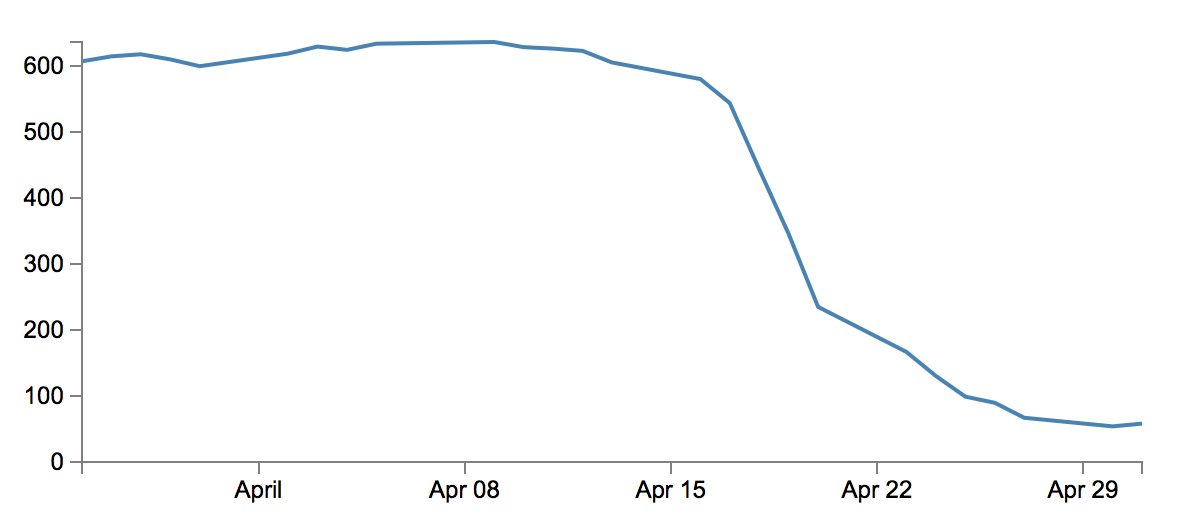
\includegraphics[scale=0.5]{graph}

In the code the dynamic properties are visible as the x- and y-axis change its parameters based on the input data. 



\chapter{Research}
\label{chp:research} 

\section{Related work}
In the last decade the importance of security against attacks on large computer systems has grown rapidly. In 2004, the ACM workshop on Visualization and data mining for computer security presented NVisionIP: netflow visualizations of system state for security situational awareness\cite{nvisionip}. This was one of the first tools too visualize NetFlow data. The visualization was based on either number of bytes transmitted or the number of flows to or from the hosts on the network. 

In \cite{nvisionip_list} they discuss the use of NVisionIP to combat different security concerns. Most of the same attacks covered in this paper are relevant today, only in today's massive amounts of data, they may be way more difficult to discover. 

\begin{itemize}
\item \textbf{Worm infection}: One of the most basic security function one might uncover.  Worms usually spread by probing for other hosts. Filtering out hosts transmitting a lot of Flows with a single destination port, one could easily see which machines are infected and should be taken offline. 
\item \textbf{Compromised systems}: If a host is compromised, the attacker might install malware that allows the attacker to control the machine. Following this an attacker might turn a host into a file server. By detecting large volumes of traffic on certain ports one might discover such an attack. 
\item \textbf{Misuse}: Misuse of computer networks in order with terms of use etc.. An example is detecting if certain users have abnormal high volumes of traffic, and by inspecting in more detail one can uncover if this trough one single application and not in accordance with the policies of the organization. 
\item \textbf{Port Scans}: When a large number of ports are used at a specific host it is easily identified by NVisionIP.
\item \label{patterns}\textbf{\gls{dos}:} Denial of Service Attacks will be visible trough spikes in traffic volume from the host attacking. If a host is attacked the same pattern is visible trough high volumes in receiving traffic. Thus peaks in traffic is not necessary an attack, but might be a result of a new release, or backup etc.
\end{itemize}




\section{Initial research}
In section \ref{netflow} we see how the raw format of the NetFlow packets look. \gls{ntnu} \gls{lvm}Comparing how understandable this format is comparing to a visual representation will be the main object of this paper(omformulere. ikke helt riktig). How much more effective is visualization compared to the raw format read by machines. 

To understand this, experiments will determine how quickly one can distinguish an attack from both the raw format, and the visual representation. 

This is were D3.js will come to great use. It can be used to quickly develop simple interactive graphs that can be used to test theories up against each other.

To be able to identify an DDoS attack, one can look at it from two angles. By finding someone whom is attacking, or someone whom is being attacked. In this case we will look at the second scenario. As mentioned earlier simply a peak in flows is not enough grounds to establish an actual attack. First of all, one will need to look for patterns of similar incidents, and what lies behind them.

\newpage

\section{Traits of a DDoS attack}
In a \gls{ddos} attack there are a large number of hosts performing the attack. In many cases a lot of them are not even aware they are a part on an attack. This is called a botnet, derived from the words robot and network. Using compromised systems, called zombies, gives the attacker control of a large enough amount of hosts to perform a volume-based DDoS attack. 

\begin{figure}[h!]
\caption{Ten files in the provided files with the most flows \citep{cisco_ddos}}
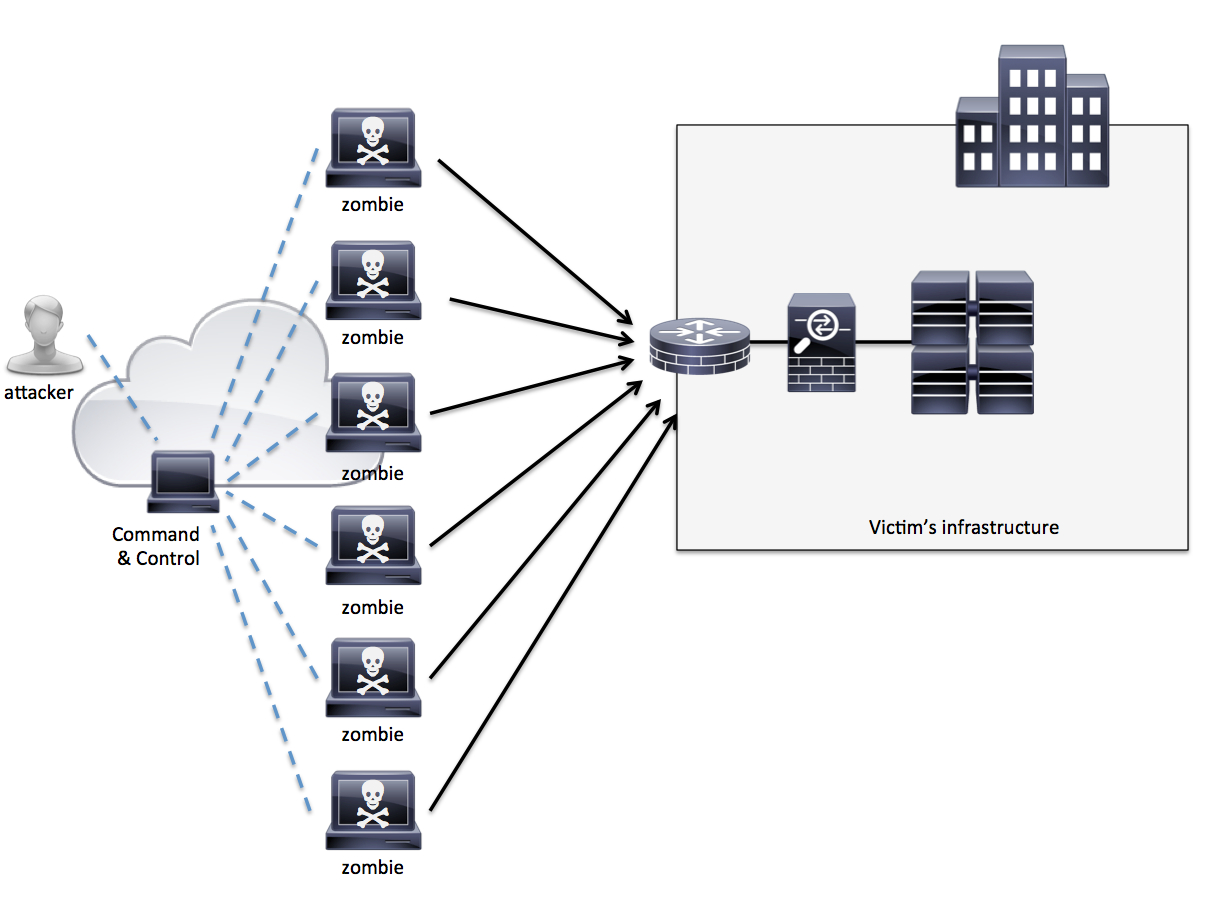
\includegraphics[scale=0.2]{botnet}
\end{figure}
Another new trend that has emerged is using large datacenters or cloud machines to launch these attacks. Either trough renting or compromising them. As cloud providers are offering such large amounts of computers, this new platform is not only great for legitimate use, but also cyber-criminals.

\begin{figure}[h!]
\caption{Ten files in the provided files with the most flows \citep{cisco_ddos}}
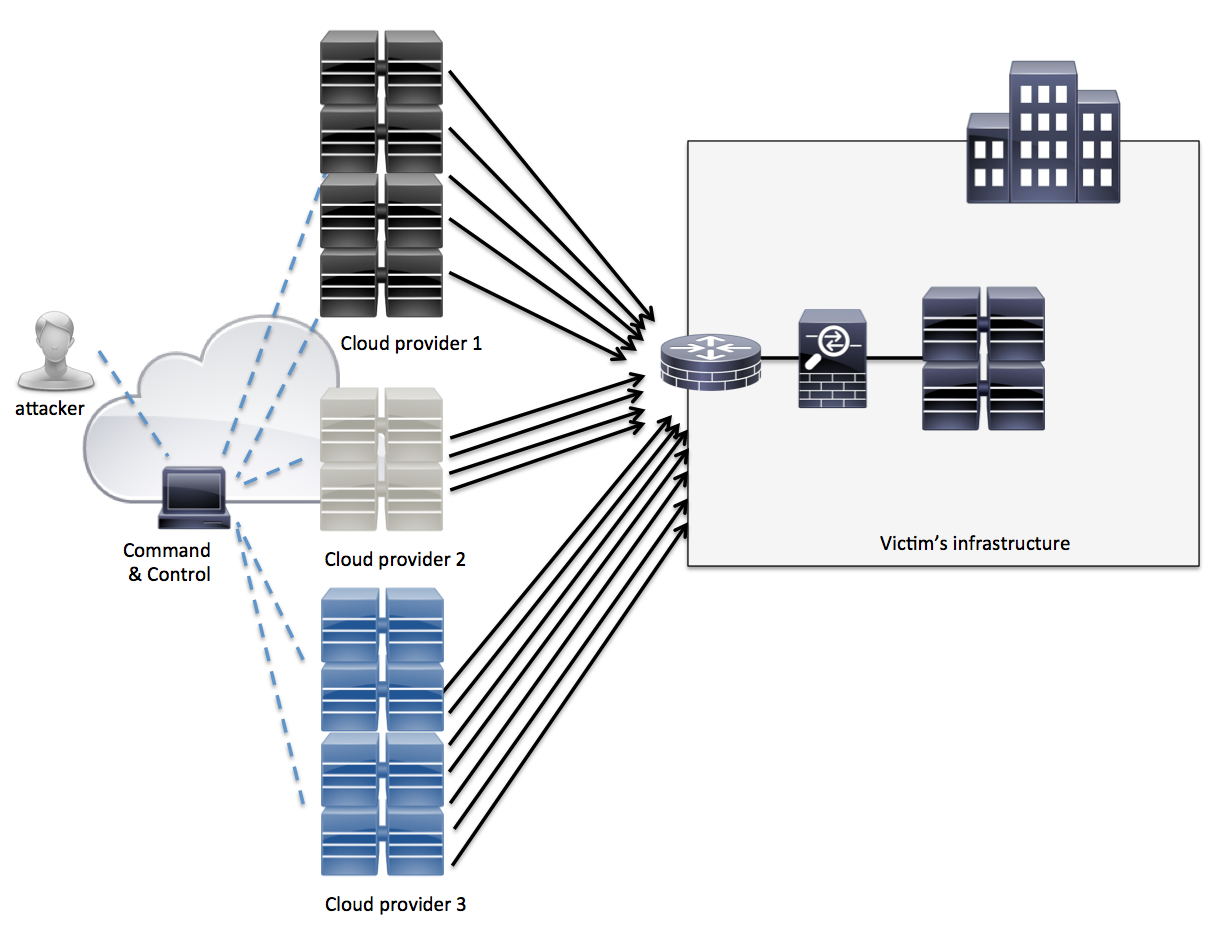
\includegraphics[scale=0.2]{cloud}
\end{figure}
Distributed Reflection Denial of Service attacks is becoming more and more popular. DrDoS techniques usually involve mulitple victim host machines that unwillingly participate in a DDoS attack on the attackers primary target. Requests to the victim host machines are redirected, or re ected, from the victim hosts to the target. Anonymity is one advantage of the DrDoS attack method. In a DrDoS attack, the primary target appears to be directly attacked by the victim host servers, not the actual attacker. This approach is called spoofing.Amplification is another advantage of the DrDoS attack method. By involving multiple victim servers, the attacker’s initial request yields a response that is larger than what was sent, thus increasing the attack bandwidth.

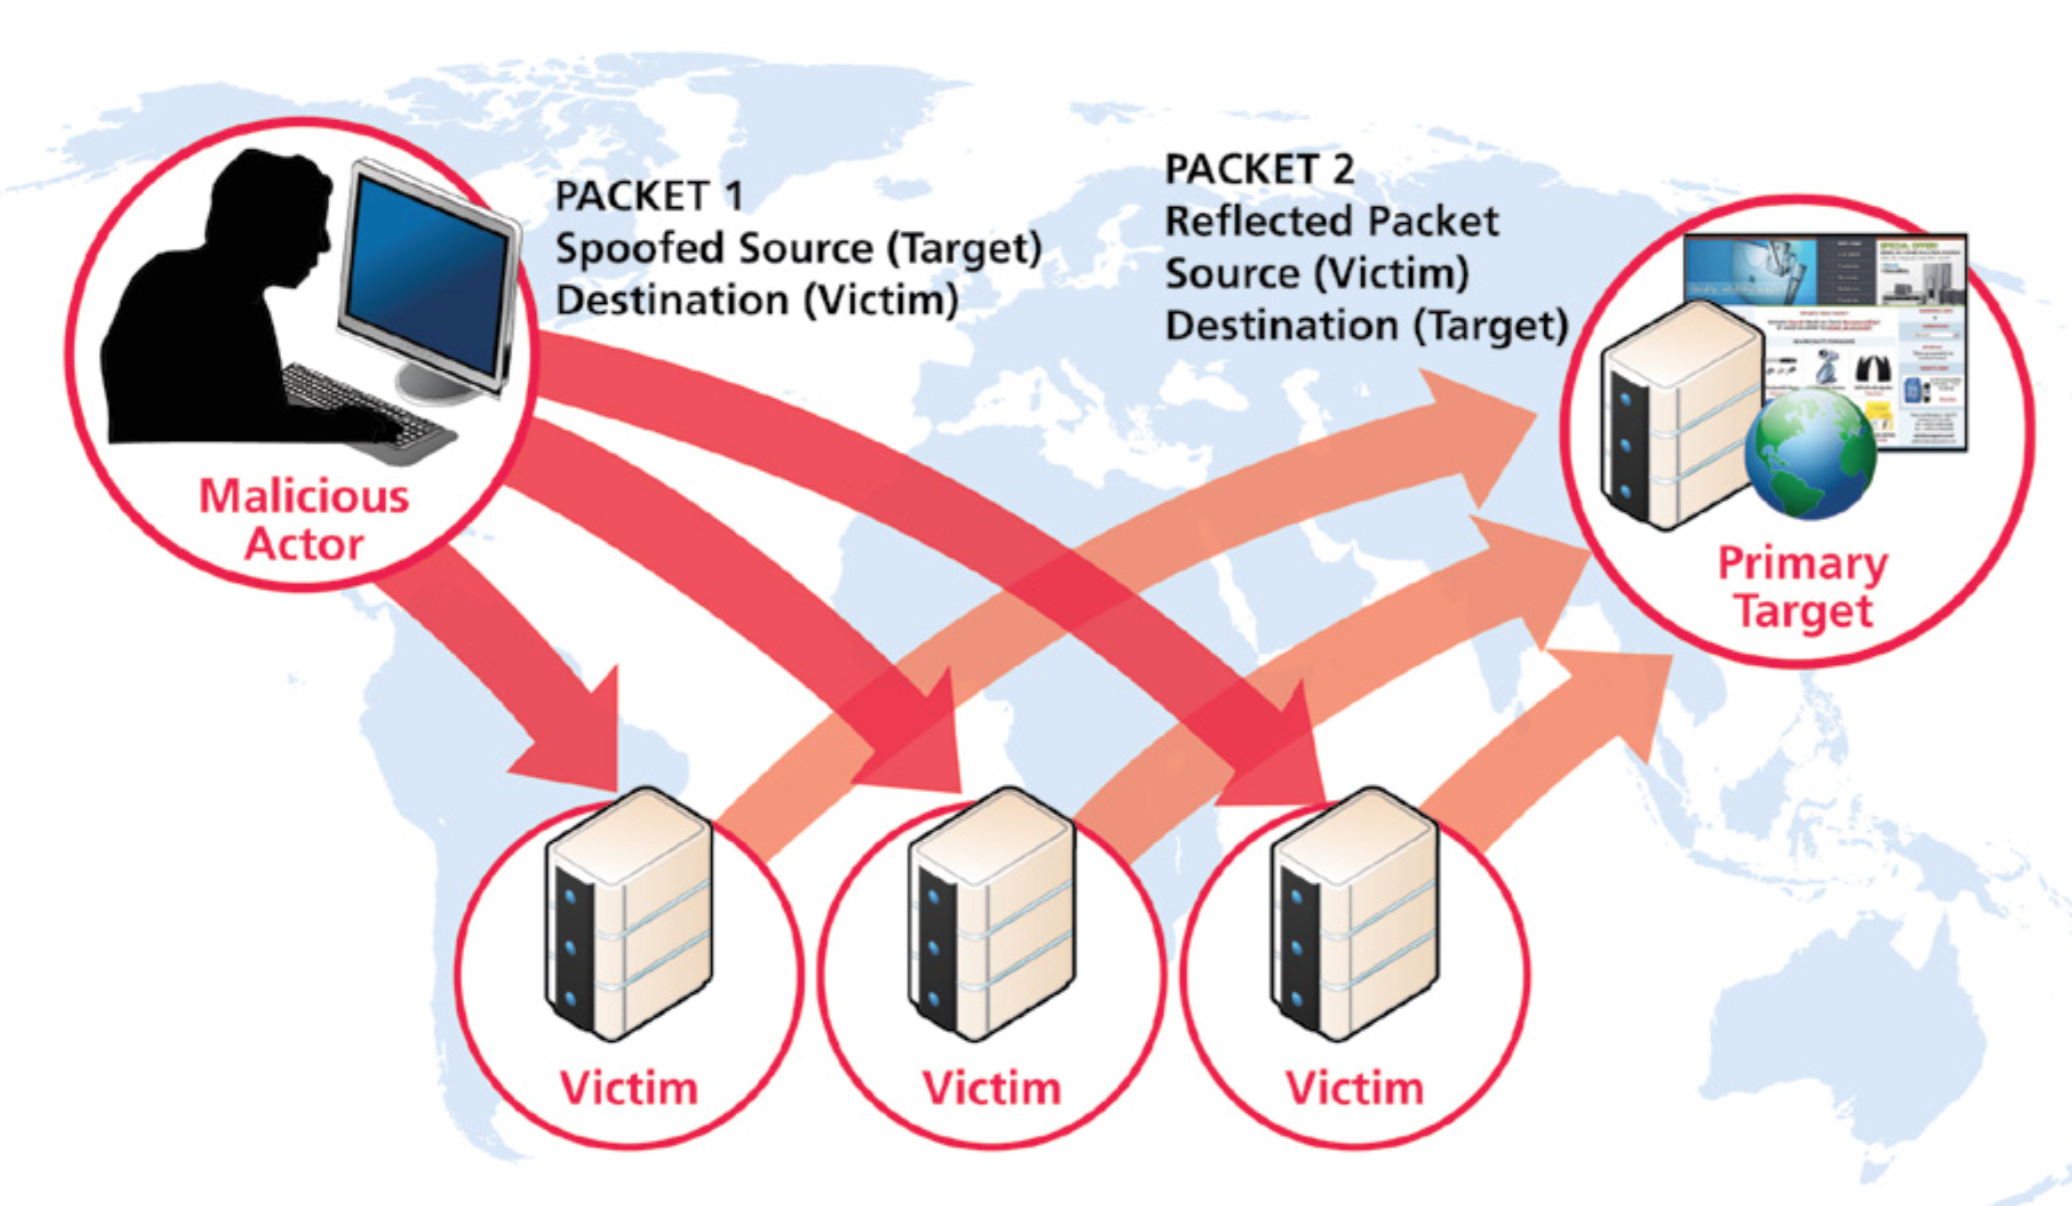
\includegraphics[scale=0.2]{drdos}

\subsection{Raw NetFlow format}

\begin{figure}[h!]
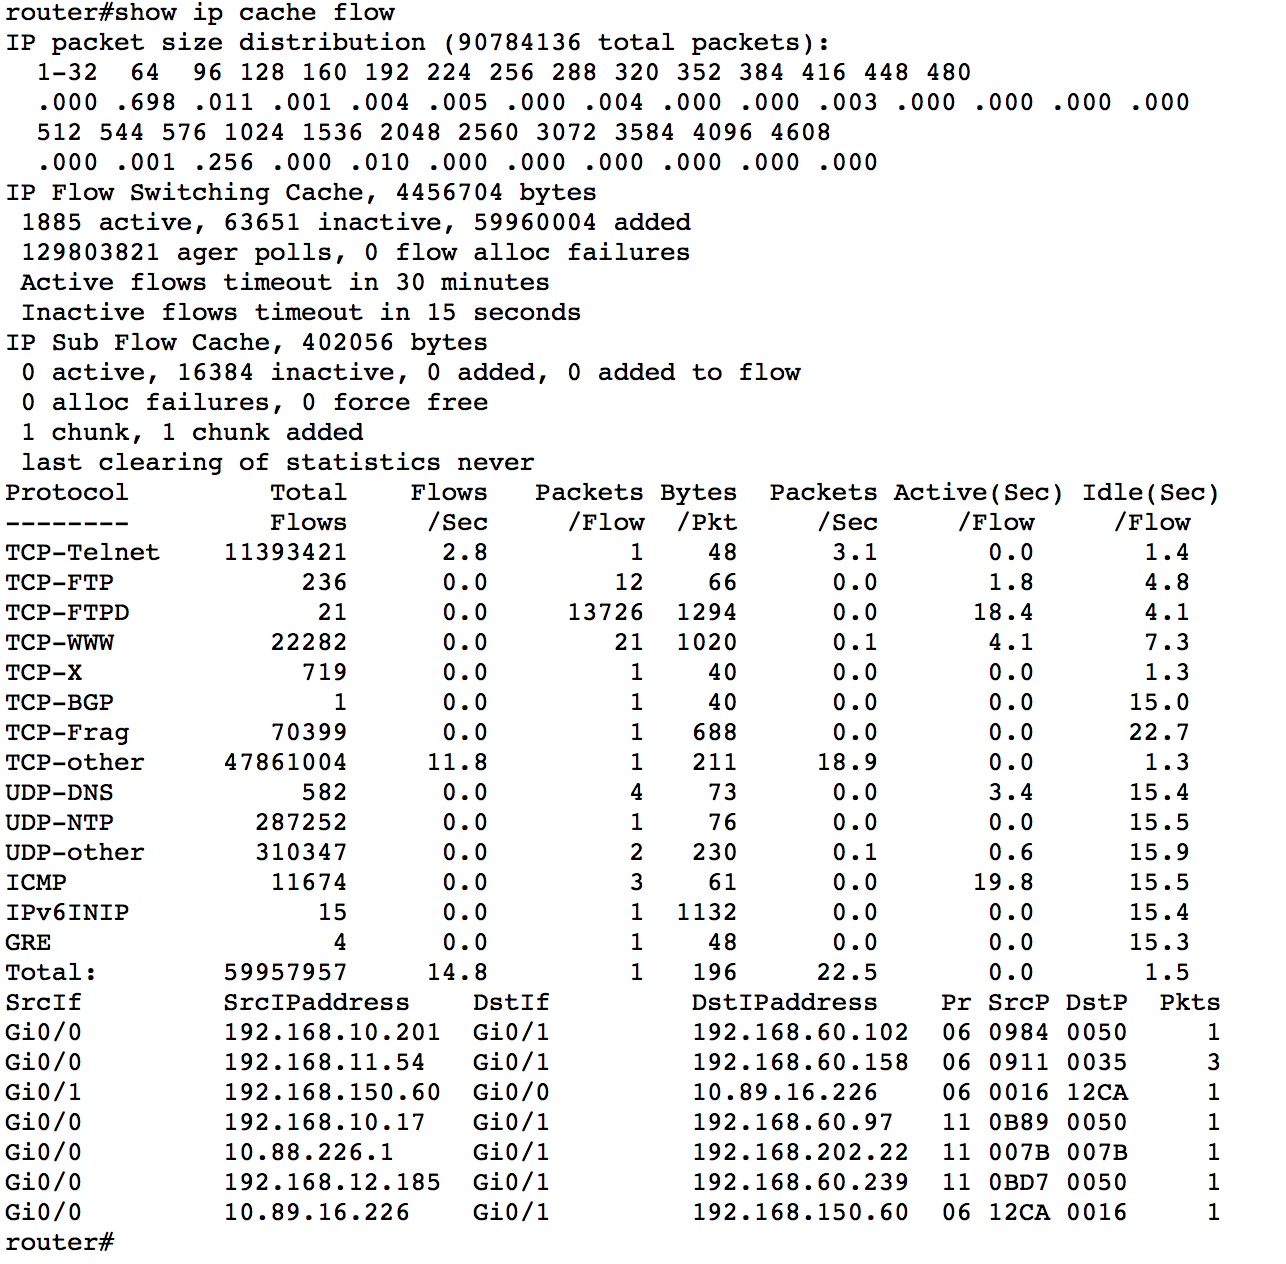
\includegraphics[scale=0.5]{netflow_ddos}
\caption{Ten files in the provided files with the most flows}
\end{figure}

In the preceding example, there are multiple flows for UDP port 80 (hex value 0050). In addition, there are also flows for TCP port 53 (hex value 0035) and TCP port 80 (hex value 0050).

The packets in these flows may be spoofed and may indicate an attempt to perform these attacks. It is advisable to compare the flows for TCP port 53 (hex value 0035) and TCP port 80 (hex value 0050) to normal baselines to aid in determining whether an attack is in progress.






\cleardoublepage
%% include here the other chapters

\renewcommand*{\bibname}{References}
\bibliographystyle{alpha}
\bibliography{main}
\listoftodos

%% Uncomment the following if you have any appendix
% \appendix
% \addtocontents{toc}{%
%  \protect\vspace{1em}% 
%  \protect\noindent \bfseries \appendixtocname\protect\par
%  \protect\vspace{-.5em}%
% }
% \renewcommand{\chaptername}{\appendixname}
%% include below possible appendices (chapters)


\end{document} 
